\documentclass[10pt]{article}
\usepackage{amssymb,amsmath,times,url,graphicx,amsthm,alltt}
%\usepackage[pdftex,urlcolor=blue,pdfpagemode=none,pdfstartview=FitH]{hyperref}
\usepackage{my_packages}
\usepackage{tikz_packages}
%% url smaller font.
\makeatletter
\def\url@leostyle{%
  \@ifundefined{selectfont}{\def\UrlFont{\sf}}{\def\UrlFont{\small\ttfamily}}}
\makeatother
\urlstyle{leo}

%\usepackage[all,import]{xy}

\renewcommand{\baselinestretch}{1.2}
\date{}

\renewcommand{\thesubsection}{\arabic{subsection}. }
\renewcommand{\thesubsubsection}{\arabic{subsection}.\arabic{subsubsection} }

\theoremstyle{definition}
\newtheorem{prob}{Problem}[section]
%\renewcommand{\theprob}{\arabic{section}.\arabic{prob}}
\renewcommand{\theprob}{\arabic{prob}}

\newenvironment{subprob}%
{\renewcommand{\theenumi}{\alph{enumi}}\renewcommand{\labelenumi}{(\theenumi)}\begin{enumerate}}%
{\end{enumerate}}%

\newenvironment{matlab}
{\begin{alltt}\small\renewcommand{\baselinestretch}{1.2}\selectfont}%
{\end{alltt}}


\begin{document}

\pagestyle{empty}
\section*{MAE3145: Homework 1}
\vspace*{-0.4cm}
\noindent{Due date: September 13, 2017}%\\%\vspace*{0.5cm}

\begin{prob}
    After a complex route to the vicinity of the moon, the two identical ARTEMIS spacecraft (P1 and P2) inserted into orbit near the Moon on August 23 and October 22, 2010, respectively. 
    The spacecraft eventually inserted into lunar orbits on June 27 and July 17, 2011.
    The trajectories in the lunar vicinity prior to the lunar orbit insertion were influenced significantly by the gravity fields of other bodies, particularly the Earth and the Sun. 
    The P1 path from arrival to the lunar insertion point appears in~\cref{fig:artemis}.
    Note that it is far from a classical elliptical orbit.
    \begin{figure}[htbp]
        \centering
        \begin{subfigure}[htbp]{0.5\textwidth} 
            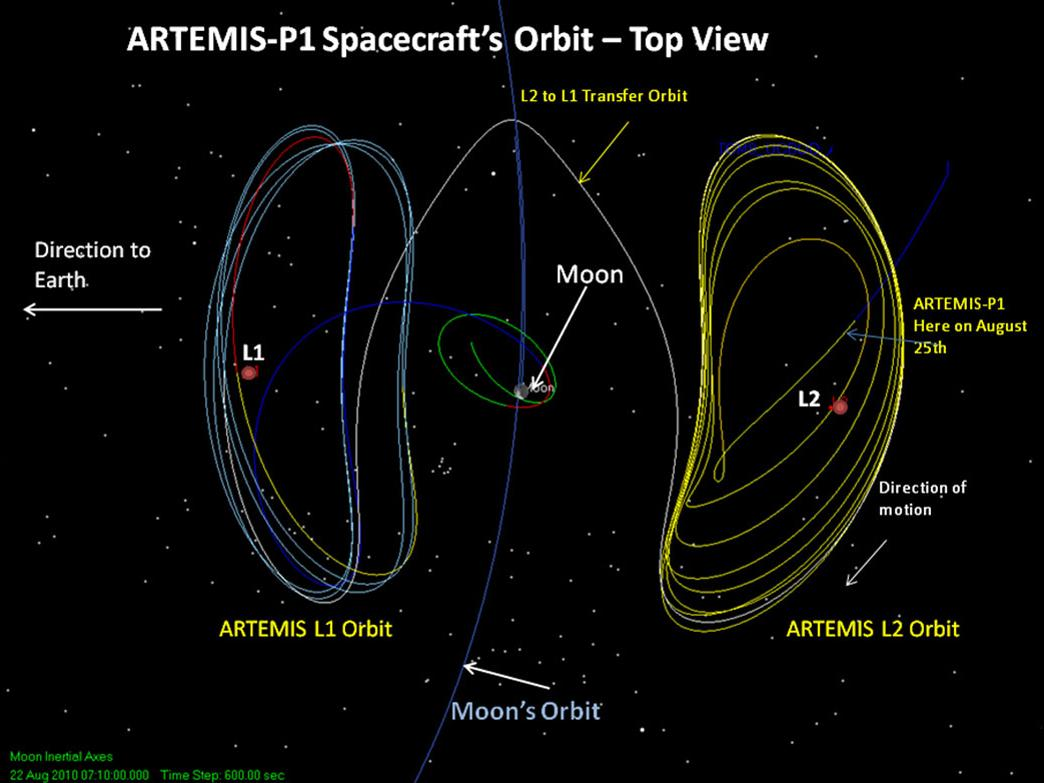
\includegraphics[width=\textwidth, keepaspectratio]{figures/artemis_top.jpg} 
            \caption{P1 Orbit top \label{fig:top_view}} 
        \end{subfigure}~
        \begin{subfigure}[htbp]{0.5\textwidth} 
            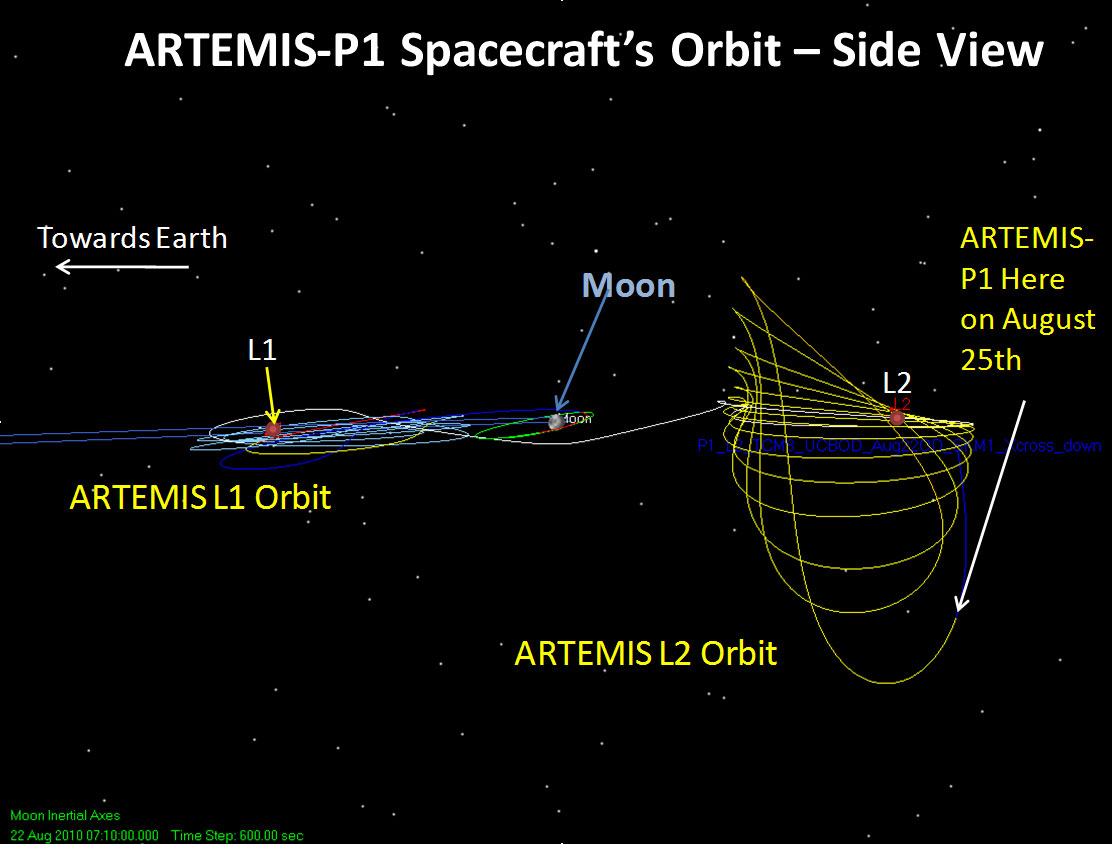
\includegraphics[width=\textwidth, keepaspectratio]{figures/artemis_side.jpg} 
            \caption{P1 Orbit side \label{fig:side_view}} 
        \end{subfigure} 
        \caption{ARTEMIS-P1 orbit~\label{fig:artemis}}
    \end{figure}
    
    Define a system that is composed of five particles.
    The law of gravity between each pair is the familiar \underline{inverse square law}.
    Obviously, the planets are not truly aligned simultaneously, but \underline{assume} that the Sun, spacecraft (s/c), and other bodies are collinear and positioned as illustrated in~\cref{fig:planets}.
    \begin{figure}[htbp]
        \centering
        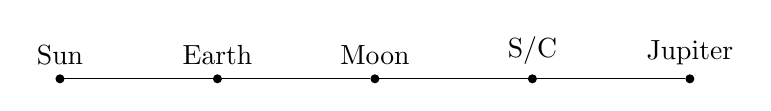
\begin{tikzpicture}
            [
            point/.style = {draw, circle, fill = black, inner sep = 1pt},
            dot/.style = {draw, circle, fill = black, inner sep = 0.2pt}
            ]
            % three corners of the triangle
            \node (s) at (0, 0) [point, label = {Sun}] {};
            \node (e) at (2, 0) [point, label = {Earth}] {};
            \node (m) at (4, 0) [point, label = {Moon}] {};
            \node (sc) at (6, 0) [point, label = {S/C}] {};
            \node (j) at (8, 0) [point, label = {Jupiter}] {};

            \draw (s) -- (e) -- (m) -- (sc) -- (j);
        \end{tikzpicture}
        \caption{Planet alignment~\label{fig:planets}}
    \end{figure}
    Assume that the spacecraft is instantaneously located such that the distance between the S/C and the Moon is \SI{150000}{\kilo\meter}.
    The total mass of each ARTEMIS space is \SI{130}{\kilo\gram}.
    The distances of the other planets from the Sun are assumed to be equal to the semi-major axis as listed on the constants handout shown on Blackboard.

    \begin{subprob}
    \item Locate the center of mass of the system. 
        Identify it on a sketch.
        Add unit vectors and the appropriate position vectors.
    \item Write the vector differential equation of motion of the S/C with respect to the center of mass, i.e. \( \bar r_i = \bar r_{s/c}\).
        You should obtain an expression for the accelerations on the S/C, i.e. \( \ddot \bar r_{s/c} = \text{sum of four terms} \).
        Assuming the alignment given in~\cref{fig:planets}, compute the accelerations on the S/C due to each of the other bodies.
        Which body produces the largest accelerations on the S/C?
        Smallest?
        What is the descending order of the accelerations due to each body?
        What is the net acceleration on the spacecraft in \si{\kilo\meter\per\second\squared}?
    \item Compare the relative magnitude of the acceleration terms on the S/C?
        Is the order of influence what you expected?
        Which gravity term dominates?
        Do the acceleration terms seem consistent with your expectations?
    \end{subprob}
\end{prob}

\begin{prob}
    Assume  that  a system is composed of three particles.
    A Hubble Space Telescope image of Pluto, and its five moons appears in~\cref{fig:pluto}.
    \begin{figure}[htbp]
        \centering
        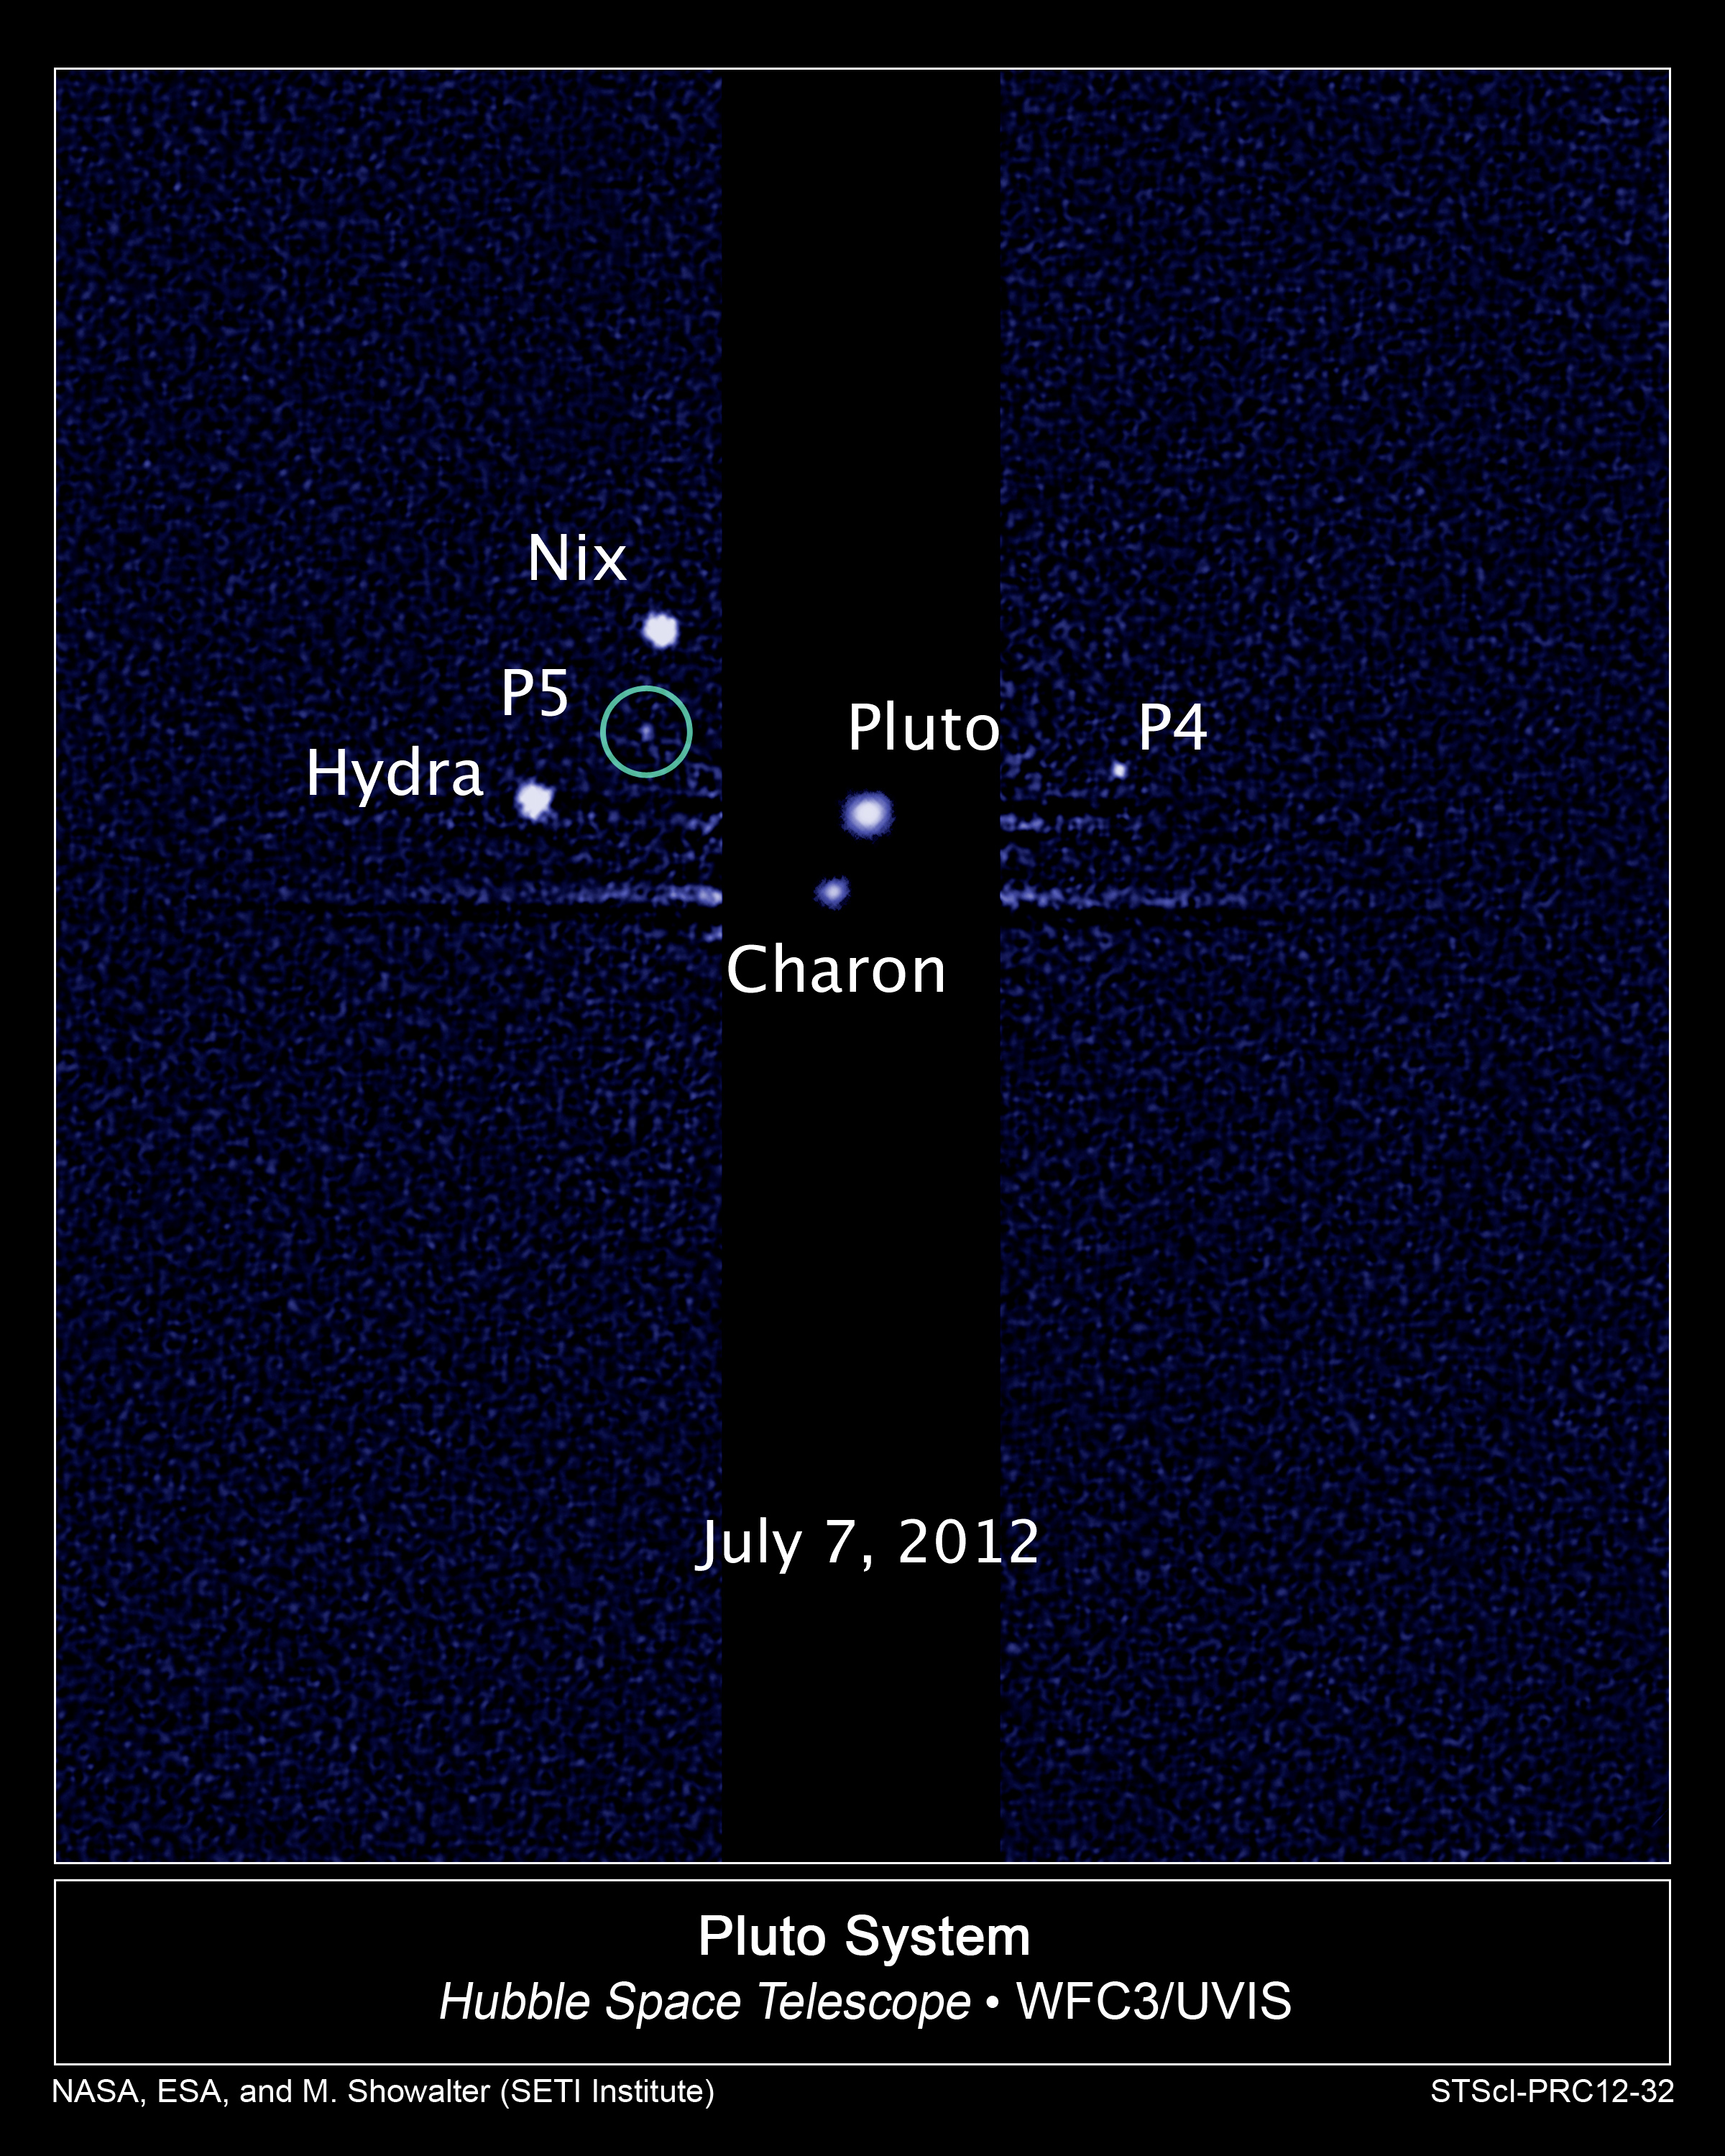
\includegraphics[trim={10cm 50cm 10cm 20cm},clip,width=0.5\textwidth]{figures/pluto.jpg}
        \caption{Pluto and moons~\label{fig:pluto}}
    \end{figure}
    Let the three particles be Pluto, Charon, and P5 (newly discovered in June 2012).
    If we want to know the orbit of the new moon, we need to write the governing differential equations.
    The law of gravitation is the familiar \underline{inverse square law}.

    \begin{subprob}
        \item Write each of the vector equations of motion that govern \( \bar r_P, \bar r_C, \bar r_{P_5} \).
            Include a sketch of the arbitrary position vectors.
        \item Add together the three second-order vector equations of motion. 
            Identify the individual terms that cancel; there should be no summation signs left in your expressions.
            Integrate this result to define the linear momentum integrals \( \bar C_1 , \bar C_2 \) for this three-body  system.
            Explain how this demonstrates that the velocity of the center of mass of this system is constant.
        \item Apply the cross product of \( \bar r_P, \bar r_C, \bar r_{P_5} \) with each equation from (a), respectively. 
            Then sum all the equations together and identify the terms that cancel. 
            Can you integrate the result?
            This procedure is the derivation of the angular moment integral \( \bar C_3\).
    \end{subprob}

    Note that the expressions for the integrals \( \bar C_1, \bar C_2, \bar C_3 \) are all functions of \( \bar r_P, \bar r_C, \bar r_{P_5} \) and \( \diff{\bar r_P}{t}, \diff{\bar r_C}{t}, \diff{\bar r_{P_5}}{t}\).
\end{prob}

\begin{prob}
    Assume that a system is composed of three particles.
    This time, let the particles be the Sun, Earth, and Moon.

    \begin{subprob}
        \item Write the \textbf{relative} vector equations of motion for the motion of the Moon relative to the Earth.
        \item Assume that the bodies are located such that they create a right triangle as shown in~\cref{fig:sem_3bp}.

            \begin{figure}[htbp]
                \centering
                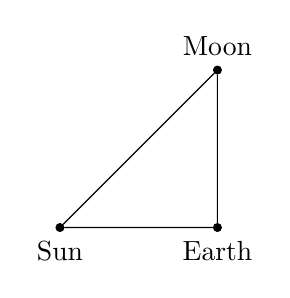
\begin{tikzpicture}
                    [
                    point/.style = {draw, circle, fill = black, inner sep = 1pt},
                    dot/.style = {draw, circle, fill = black, inner sep = 0.2pt}
                    ]

                    \node (s) at (0, 0) [point, label = below:{Sun}] {};
                    \node (e) at (2, 0) [point, label = below:{Earth}] {};
                    \node (m) at (2, 2) [point, label = above:{Moon}] {};

                    \draw (s) -- (e) -- (m) -- (s);
                \end{tikzpicture}
                \caption{Sun, Earth, Moon three body system~\label{fig:sem_3bp}}
            \end{figure}

            Compute the dominant and perturbing accelerations on the Moon.
            Use the information provided in the table of constants on Blackboard. 
            By comparing the magnitudes, is it reasonable to model the Moon's motion using only the gravity of the Earth (two body problem)?
            Why or why not?
            Will the solar gravity have a significant influence?

        \item Is a two-body model (Earth and Moon) reasonable for the motion of the Moon?
    \end{subprob}
\end{prob}
\begin{prob}
The motion of two point masses acting under their mutual gravity is described, with respect to an inertial frame, by the following set of ordinary differential equations.
\begin{align}
m_1\ddot{{R}}_1 & = G \frac{m_1 m_2}{r^2} \hat u_r,\\
m_2\ddot{{R}}_2 & = -G \frac{m_1 m_2}{r^2} \hat u_r,
\end{align}
where $ r= R_2 - R_1$, $r=\norm{ r}$, $\hat u_r = \frac{ r}{r}$. Suppose that the units are normalized such that $m_1=2\,\mathrm{kg}$, $m_2=1\,\mathrm{kg}$, $G=1\,\mathrm{m^3/kg s^2}$.

The initial conditions are given by
\begin{align*}
 R_1(0)&=[0,0,0]^T\,(\mathrm{m}), \qquad  V_1(0)=[0,0,0]^T\,(\mathrm{m/s}),\\
 R_2(0)&=[1,0,0]^T\,(\mathrm{m}), \qquad  V_2(0)=[1,1,0]^T\,(\mathrm{m/s}).
\end{align*}
We wish to compute the resulting trajectories of $m_1$ and $m_2$ using Python. 


First, we rewrite the equations of motion as the standard form of $\dot x = f(t,x)$. Let the state vector be $x=[R_1^T,\,V_1^T,\, R_2^T,\, V_2^T]\in\Re^{12}$. The equations of motion can be rewritten as
\begin{align}
\begin{bmatrix} \dot R_1 \\ \dot V_1 \\ \dot R_2 \\ \dot V_2\end{bmatrix}
=
\begin{bmatrix}
V_1 \\
G\frac{m_2}{r^2} \hat u_r\\
V_2 \\
-G\frac{m_1}{r^2} \hat u_r
\end{bmatrix}.
\end{align}


\begin{subprob}

\item Write a Python function, namely \texttt{eomTBI} that returns $\dot x$ for given $(t,x)$. This function will be used by the \texttt{scipy.integrate.odeint} integrator.

You should test that your function is correct.
Decide on a sequence of unit tests that will ensure your function is correct. 
For example, for the initial conditions given above, your function should return 
\begin{align}
    \dot{x} = \begin{bmatrix} 0 , 0 , 0 , 1 , 0 , 0 , 1 , 1 , 0 , -2 , 0 , 0 \end{bmatrix} .
\end{align}


\item Write a Python script, entitled \texttt{simTBI.py} to obtain $R_1(t), R_2(t)$ using \texttt{scipy.integrate.odeint}, and plot the trajectories of $m_1$, $m_2$ together on a single $xy$ plane (The $x$ axis is for the $x$-component of $R_1,R_2$, and the $y$ axis is for their $y$ components. There is no need to plot the $z$-components, as they are identical to zero). The simulation time is $0\leq t \leq 10$ seconds.

\item The position of the mass center of two point masses is given by
\begin{align*}
 R_G = \frac{m_1  R_1 + m_2  R_2}{m_1+m_2}.
\end{align*}
Compute the trajectory of the mass center using the results of (d) and plot it on the $xy$ plane.


%\item Since the acceleration of the mass center is zero, the position of the mass center can also be obtained by the following equation.
%\begin{align*}
% R_G (t) =  R_G (0) +  V_G(0) t.
%\end{align*}
%Compute $R_G(10)$ by hands using the above equation, and check that it is consistent with your solution of (e).
\item The relative position of $m_2$ from $m_1$ is given by
\begin{align*}
 r =  R_2 - R_1.
\end{align*}
Compute the trajectory of the relative motion, and plot it on the $xy$ plane.

\end{subprob}
\end{prob}


\begin{prob}
    Consider the N-body problem

    Create a simulation  of the solar system

    Here are the initial conditions for the solar system at some epoch,

    Here is where they should be in 1 year, find where they are in on your next birthday
    
    Show a plot and normalize by Earth orbit to get AU
\end{prob}

\begin{prob}
    Some problems from BMW chapter 1, compute energy, angular moment, and other constants for orbiting bodies

    problems from vallado
\end{prob}
\end{document}




% \begin{prob}
% The relative motion of two point masses acting under their mutual gravitational potential is described by the following ordinary differential equation.
% \begin{align}
% \ddot{ r} = -\mu \frac{ r}{r^3},
% \end{align}
% where $\mu=G(m_1+m_2)$.
% \begin{subprob}
% \item Write a Matlab code to solve this equation for $ r(t)$, and plot the relative trajectories on the $xy$ plane for the following initial conditions. The properties of two masses and the simulation time are the same as Problem 1.
% \begin{align*}
%  r(0)=  R_2(0)- R_1(0) = [1,0,0]^T\,(\mathrm{m}), \qquad 
%  v(0)=  V_2(0)- V_1(0) = [1,1,0]^T\,(\mathrm{m/s}).
% \end{align*}
% \item Check that your solution of \textbf{Problem 2}.(b) is consistent with \textbf{Problem 1}.(d).
% \end{subprob}
% \end{prob}


% \clearpage\newpage
% \section*{MATLAB: Initial Value Problem for Ordinary Differential Equations}

% Consider an ordinary differential equation
% \begin{align}
% \dot x = f(t,x),\label{eqn:f}
% \end{align}
% where $x\in\Re^n$, $f:\Re\times\Re^n\rightarrow\Re^n$. An initial value problem is to find the solution $x(t)$ satisfying the ordinary differential equation and an initial condition $x(0)=x_0$. Matlab provides several solvers for initial value problems. Here, we show an example for a pendulum. 

% \paragraph{Pendulum Model} A pendulum is a point mass connected to a frictionless pivot point by a massless link acting under gravity. The motion of a pendulum is described by the following differential equation.
% \begin{align}
% \ddot \theta = - \frac{g}{l} \sin\theta,\label{eqn:ddottheta}
% \end{align}
% where $\theta$ is the angle of the link from the hanging position, $l$ is the length of the link, and $g$ is the gravitational acceleration.

% We will solve an initial value problem of this pendulum model using the Matlab \texttt{ode45} function. The initial conditions and the properties of the pendulum is given by
% \begin{align*}
% \theta(0)=\frac{\pi}{4},\quad \dot\theta(0)=0,\quad l=9.81\,\mathrm{m},\quad g=9.81\,\mathrm{m/s^2}.
% \end{align*}

% \paragraph{Step 1. Standard First-Order Form} The first step is to rewrite the differential equation \refeqn{ddottheta} into the standard first-order form \refeqn{f}. Define
% \begin{align}
% x_1=\theta,\quad x_2=\dot\theta.
% \end{align}
% Then, \refeqn{ddottheta} can be written as two-dimensional first-order differential equations of a state vector $x=[x_1,x_2]^T\in\Re^2$.
% \begin{align}
% \dot x_1 & = \dot\theta = x_2,\\
% \dot x_2 & = \ddot\theta = -\frac{g}{l}\sin\theta = -\frac{g}{l}\sin x_1.
% \end{align}
% These equations can be rewritten as
% \begin{align}
% \dot x = \begin{bmatrix} \dot x_1 \\ \dot x_2 \end{bmatrix}
% =\begin{bmatrix} x_2 \\ -\frac{g}{l} \sin x_1\end{bmatrix}=f(t,x),
% \end{align}
% which has the same form as \refeqn{f}.

% \paragraph{Step 2. Matlab Function for $f$} The next step is writing a Matlab function m-file for $f(t,x)$: the input of this function is a time $t$ and a state vector $x$, and the output is $\dot x$. The following Matlab m-file function represent the equation of motion for a pendulum. Note that it should be saved as \texttt{eomPend.m}.

% \begin{alltt}
% \footnotesize\renewcommand{\baselinestretch}{1.2}\selectfont
% function dotX=eomPend(t,X)
% g=9.81;
% l=9.81;

% theta=X(1);
% dottheta=X(2);

% ddottheta=-g/l*theta;

% dotX=[dottheta; ddottheta];
% \end{alltt}

% \paragraph{Step 3. Use \texttt{ode45} Function} The Matlab function \texttt{eomPend.m} is integrated by the Matlab initial value problem solver \texttt{ode45}. The syntax is as follows

% \begin{alltt}
% [t,X] = ode45(@odefun,tspan,X0);
% \end{alltt}
% where \texttt{@odefun} is the handle of the differential equation, \texttt{tspan=[t0 tf]} specifies the simulation time for the initial time \texttt{t0} and the terminal time \texttt{tf}. The initial condition is specified by \texttt{X0}. Then, it returns the column vector \texttt{t} of time points, and the solution array \texttt{X}, where each row in \texttt{X} corresponds to the solution at a time returned in the corresponding row of \texttt{t}.

% For our initial value problem for the pendulum, use the following Matlab script m-file.
% \begin{alltt}\footnotesize\renewcommand{\baselinestretch}{1.2}\selectfont
% clear all;
% close all;

% theta0=pi/4;
% dottheta0=0;
% X0=[theta0; dottheta0];

% [t,X]=ode45(@eomPend,[0 10],X0);

% theta=X(:,1);
% dottheta=X(:,2);

% plot(theta,dottheta);
% \end{alltt}
% \end{document}

